\documentclass[11pt]{article}  % required first line, though can vary;
                               % this says we will use 11-point font,
                               % in the "article" format
\usepackage{mathtools}
\usepackage{listings}
\usepackage{graphicx}
\graphicspath{{image/}}

%\DeclareGraphicsExtensions{.jpg}


% these \setlength etc. lines concern page layout, amount of paragraph
% indentation etc.; beginners should ignore them (but include them)
\setlength{\oddsidemargin}{0.0in}
\setlength{\evensidemargin}{0.0in}
\setlength{\topmargin}{-0.25in}
\setlength{\headheight}{0in}
\setlength{\headsep}{0in}
\setlength{\textwidth}{6.5in}
\setlength{\textheight}{9.25in}
\setlength{\parindent}{0in}
\setlength{\parskip}{2mm}

\begin{document}
\begin{center}
\textbf{Project Forestcover}\\

Team Members
\line(1,0){500}
\end{center}
\section*{Part 1}




\subsection*{Exponential cost function}

\subsection*{1. Choice of the Heuristic Functions}
For cost function $c_{1} = e^{(h_{2}-h_{1})}$, we choose heuristic functions as follows:

Let $K$ be a constant, defined as equal to $0$ if $\Delta d \le |\Delta h|$, and equal to $\Delta d - |\Delta h|$ otherwise.

\begin{itemize}
\item Case 1: if $\Delta h < 0$, and $\Delta d > |\Delta h|$
\begin{equation}
h = \left| \Delta h \right |*e^{-1} + K
\end{equation}

\item Case 2: if $\Delta h = 0$
\begin{equation}
h = \Delta d + K
\end{equation}

\item Case 3: if $\Delta h > 0$, and $\Delta d \leq \left | \Delta h \right |$
\begin{equation}
h = \left| \Delta h \right |*e + K
\end{equation}

\item Case 4: This is a special case, so we discuss it seperately. If $\Delta h < 0$, and $\Delta d < |\Delta h|$
\begin{equation}
h = \Delta d * e^\frac{\Delta h}{\Delta d} + K
\end{equation}

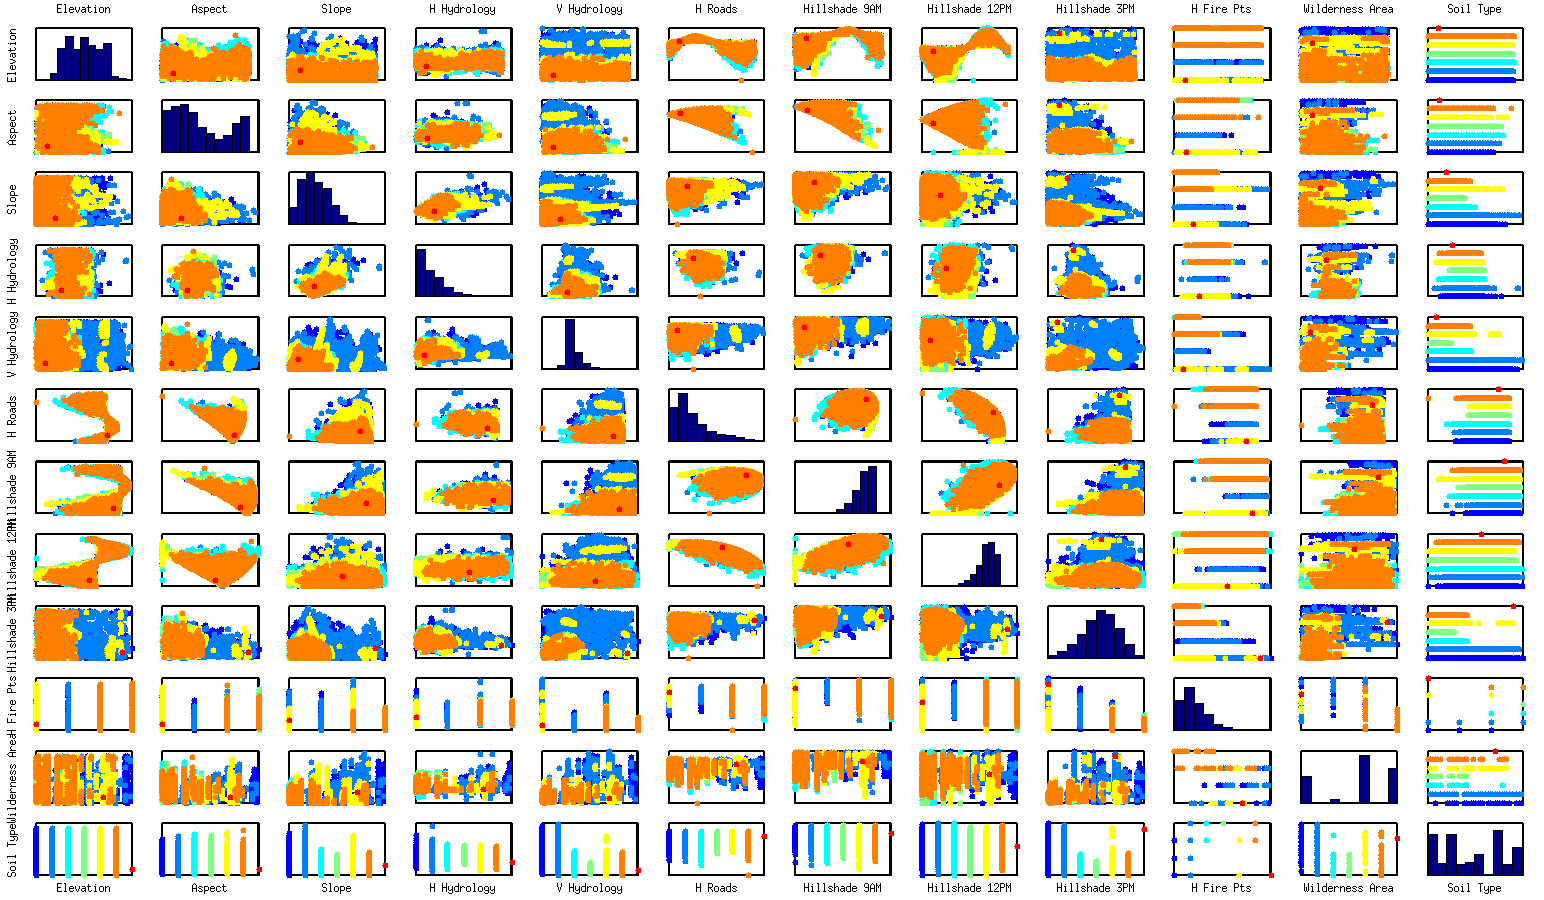
\includegraphics[scale=0.4]{featureScatterPlotMatrixHD}
\end{itemize}


\subsection*{2. Proof of the heuristic functions}
\begin{itemize}
\item Choice of K: Without the constant $K$, the heuristic function represents the minimal cost to go from $p_1$ to $p_2$ if the magnitude of $\Delta d$ is less than or equal to $\Delta h$. In other words, the function underestimates the cost to change our altitude from $p_1$'s height to that of the goal state. But that minimal change occurs in a number of steps less than the magnitude of $\Delta h$. So, without $K$, in all cases our function is a true underestimate, but by adding $K$ (with a value greater than $0$ when our goal is further away in horizontal distance than it is in height difference) we obtain a larger underestimate, which takes into account the need to travel an additional amount after the goal height has been reached. Case 2 of this proof provides more detail as to why the remaining distance to the goal is an acceptable underestimate.
\item Case 1: As with case 3, by comparing the geometric mean and arithmetic mean of the optimal path from $p_1$ to $p_2$, we obtain a function which provides a lower bound on the cost of an optimal path to the goal. This function is minimized when the number of steps is equal to the negative of $-\Delta h = |\Delta h|$ (because the absolute value of a negative number is the negation of that number). Thus by the same equation as in case 1, we obtain $\Delta h \times e^\frac{\Delta h}{|\Delta h|} = \Delta h \times e^{-1}$.

\item  given by $\Delta d * e^{0} = \Delta d$, which is the cost of going from $p_1$ to $p_2$ without any change in elevation, is an underestimate of the true cost. 
\item Case 3: Let the true cost from $p_1$ to goal be $C$, and it takes $x$ moves to reach the goal; let $h_i$ be the height of nodes along this path; let $h_x$ be the height of the xth node, i.e. goal node. (We use $h_2$ for the height of goal in other cases, but in this case, $h_2$ is the height of 2nd node along this path, as $h_i$ is the ith node alone this path)
\begin{align}
C &= \underbrace{e^{h_2-h_1}+e^{h_3-h_2}+e^{h_4-h_3} + ... + e^{h_x-h_{x-1}}}_{\mbox{total of $x$ terms}}\\
&> x \sqrt[x]{e^{h_2-h_1} \times e^{h_3-h_2} \times e^{h_4-h_3} \times ... \times e^{h_x-h_{x-1}}}\\
&= x \sqrt[x]{e^{h_2-h_1+h_3-h_2+h_4-h_3 +... +h_x-h_{x-1}}}\\
&= x \sqrt[x]{e^{h_x-h_1}}
\end{align}
But $h_x - h_1$ is $\Delta h$, so let $F$ be a function of $x$.
\begin{center}
$F(x) = x \sqrt[x]{e^{\Delta h}}$
\end{center}
and F(x) is a lower bound of the true cost $C$. We want to know the minimum value of this function F to get an lower bound of F, and this minimum value is apparently admissible, thus we can use it as our heuristic function. We simply need to take derivative of $F$ to obtain the minimum value.
\begin{center} 
$\frac{d}{dx} F(x) = \frac{d}{dx} x \sqrt[x]{e^{\Delta h}} = 0 $
\end{center}
gives when $x=\Delta h$, $F$ has minimum value. Thus
\begin{center} 
$F_{min} = \Delta h  \sqrt[\Delta h]{e^{\Delta h}} = \Delta h \times e$
\end{center}
and this is the heristic function when $\Delta h > 0$. 

For case 1, we use same process, but $\Delta h$ is a negative number. Thus F has minimum when $x=-\Delta h$ since $x$, the number of moves, must be a positive number, so we get
\begin{center} 
$F_{min} = |\Delta h|  \sqrt[|\Delta h|]{e^{\Delta h}} = \Delta h \times e^{-1}$
\end{center} 
and these two heuristic functions are guaranteed to be the smallest cost, thus admissible.



\item Case 4:
Because we are going downhill by a number of steps less than the height difference between $p_1$ and $p_2$. The minimum cost to $p_2$ is obtained by a direct route of $\Delta d$ steps at a steady downward pace. The negative exponent is equal to the average height decrease necessary to reach $p_2$'s height. Because this combination of factors maintains the smallest average step cost (going downhill each time) and the minimal number of steps (exactly equal to our diagonal distance from $p_1$ to $p_2$), this represents the absolute minimum cost to reach $p_2$ and thus is an underestimate of the true cost.

\end{itemize}


\subsection*{Ratio cost function}
\subsection*{1. Choice of the Heuristic Functions}
For cost function $c_{2} = \frac{h_{2}}{h_{1} + 1}$, we choose heuristic funtions as follows:
\begin{itemize}
\item Case 1: if $\Delta d = 0$
\begin{equation}
h = 0
\end{equation}
\item Case 2: if $\Delta d = 1$
\begin{equation}
h=\frac{h_2}{h_1+1}
\end{equation}
\item Case 3: if $h_1 \le 1$
\begin{equation}
h=\Delta d * 0.5
\end{equation}
\item Case 4: if $\Delta d \ge h_1$
\begin{equation}
h= \log h_1 + \frac{h_1}{2} - \frac{1}{2} + \frac{\Delta d - h_1}{2}
\end{equation}
\item Case 5: Otherwise
\begin{equation}
h= \log \Delta d - \frac{1}{2} + \frac{\Delta d}{2}
\end{equation}


\end{itemize}

\subsection*{2. Proof of the Heuristic Functions}
General Description of Heuristic Philosophy: We relax the cost of climbing in height by allowing any increase in height to cost exactly 1. This is a lower bound on the cost of an upward step by our cost function, so this is always an underestimate of the true cost of an upward climb. Because the cost of upward movement is essentially nullified with this relaxation, in every case the optimal path is a combination of descent from our current height, coupled with, if further distance remains to be travelled, horizontal movement at a height of 1 (the lower we are, the cheaper is to move and maintain the same height, and our data is provided with the stipulation that no adjacent tiles have a height of 0).
\begin{itemize}
\item Case 1: If we are at the goal, the heuristic returns an estimate of 0.
\begin{center}
$\frac{1}{2}+\frac{1}{3}+\frac{1}{4}+ ... +\frac{1}{n+1} = \sum_{i=1}^{n+1}\frac{1}{i}$
\end{center}
\item Case 2: The goal is one step away. The minimal cost to get there is to go there.
\item Case 3: Our current height is already minimal, so the optimal path from $p_1$ to $p_2$ (remembing our relaxation which says that it costs us nothing to climb in the last step to the goal's height) is to continue to travel at a height of 1 until we reach the goal's tile. Since this cost would only hold on a real map if the goal's height was also 0 or 1, this is an underestimate of the true cost.
\item Case 4: We are at a height greater than 1 and our height is greater than our horizontal distance to the goal. The optimal strategy is some combination of gradual (or not so gradual) descent coupled with lateral movement at a height of 1. We cannot descend all the way to our goal, because each descent decreases our elevation by 1 and our elevation is less than the distance to the goal. So we underestimate the cost of descending to ground level by assuming that we make $h_1$ steps, all of which have an absolute minimum cost of $\frac{1}{h_c+1}$, where $h_c$ is our height at that stage of our descent.

For example, if we start at height 10, and we will ultimately have to travel 50 tiles to reach our goal, we can descend for at most 10 tiles. From height 10, the minimal cost of descent is $\frac{1}{11}$. We underestimate the total cost of descent by allowing that cost, which would actually take us to an elevation of 1, to represent the cost of travelling 1 tile closer to our goal but remaining at a height of 9 (the longer we can stay elevated, the longer we can descend and incur costs less than one half, which we will be forced to accept once we have reached the bottom elevation). Staying elevated, since we are underestimating by using 1 always in the numerator, will allow each lateral step to have a cost equal to $\frac{1}{h_c+1}$, which is always less than one half. We could simply multiply $h_1$ by $\frac{1}{h_1+1}$, but by allowing the denominator to decrease gives us a larger underestimate and is hence preferable.

So, the underestimated cost of descending from height 10 while moving laterally 10 tiles is equal to the sum of $\frac{1}{11} + \frac{1}{10} + \frac{1}{9} + ... + \frac{1}{2}$. This can be recognized as the first $h_1$ terms of the harmonic series. A lower bound on the partial sums of the harmonic series is given by: $\log n + \frac{1}{2n} - \frac{1}{2} \ge \log n - \frac{1}{2}$, which is the bound used to provide our underestimate of the cost of descent.

This underestimate is generally far less than the true cost, but it has the advantage of being in all cases less than or equal to the true cost, and thus admissible.
\item  Case 5: This case is essentially the same as the previous case, except that our lateral distance to travel is less than our current height, so the minimal number of steps is equal to $\Delta d$, not $h_1$, and thus we consider only the first $\Delta d$ terms of the harmonic series in calculating our lower bound.
\end{itemize}




\end{document}
